
\subsection{Preprocessamento dos dados de Material Particulado (MP-10)}

A Figura \ref{fig:data-pm10-raw} mostra a série temporal do sensor de \acrshort{mp10} depois de removidos os valores fora de intervalo. Os resultados do pré-processamento das leituras do sensor são ilustrados nas Figuras \ref{fig:data-pm10-preproc-hist} e \ref{fig:data-pm10-preproc-15} que apresentam, respectivamente, o histograma dos dados e a série pré-processada do sensor OPC-N3 juntamente com o comportamento diário das medições ao longo do período sob análise agrupados por hora do dia. Os dados foram re-amostrados para um período de 1 hora para serem calibrados com as leituras de referência, a Figura \ref{fig:data-pm10-preproc-1HR} mostra a série temporal resultante da re-amostragem.

\begin{figure}[h]
    \centering
    \caption{Série temporal das leituras do sensor OPC-N3}
    \begin{subfigure}{0.495\textwidth}
        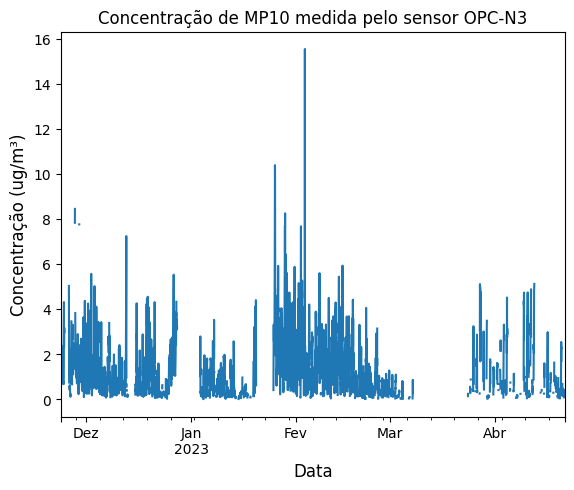
\includegraphics[width=\textwidth]{chapters/3-ANÁLISE DOS DADOS/Figuras/raw-pm10.png}
        \caption{Série temporal do sensor depois de remover valores fora de intervalo}
        \label{fig:data-pm10-raw}
    \end{subfigure}
    \hfill
    \begin{subfigure}{0.495\textwidth}
        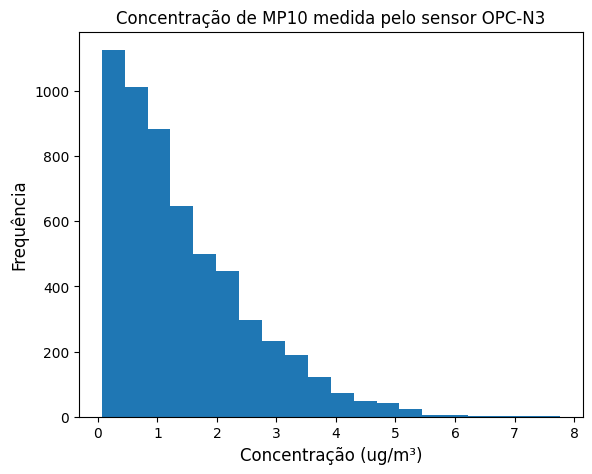
\includegraphics[width=\textwidth]{chapters/3-ANÁLISE DOS DADOS/Figuras/preproc-hist-pm10.png}
        \caption{Histograma das leituras pré-processadas do sensor OPC-N3}
        \label{fig:data-pm10-preproc-hist}
    \end{subfigure}
    \begin{subfigure}{0.99\textwidth}
        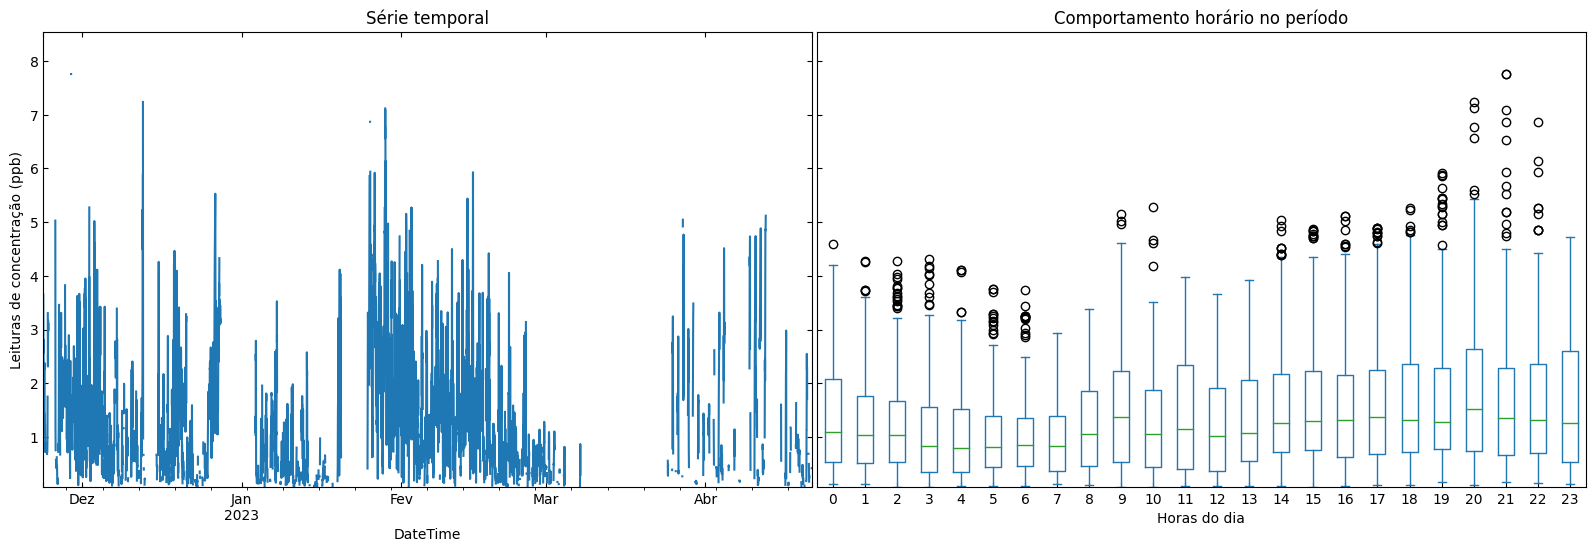
\includegraphics[width=\textwidth]{chapters/3-ANÁLISE DOS DADOS/Figuras/preproc-pm10.png}
        \caption{Série temporal do sensor pré-processada (T = 15 mins) e seu comportamento diário}
        \label{fig:data-pm10-preproc-15}
    \end{subfigure}
    \hfill
    \label{fig:data-pm10-15}
    \fonte{Desenvolvido pelo autor (2023)}
\end{figure}

\begin{figure}[h]
    \centering
    \caption{Série temporal horária das leituras do sensor OPC-N3 e sua relação com a temperatura}
    \begin{subfigure}{0.495\textwidth}
        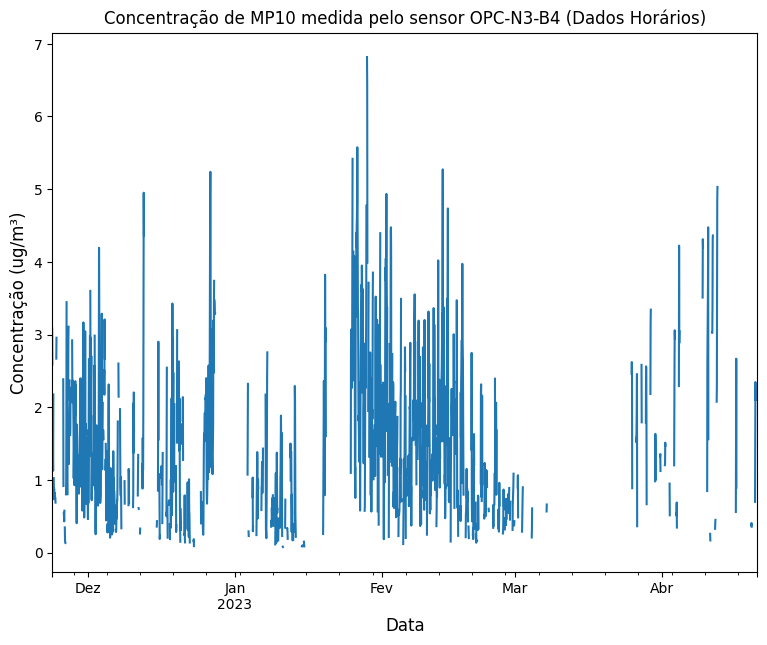
\includegraphics[width=\textwidth]{chapters/3-ANÁLISE DOS DADOS/Figuras/preproc-1HR-pm10.png}
        \caption{Série temporal com T = 1 hr}
        \label{fig:data-pm10-preproc-1HR}
    \end{subfigure}
    \hfill
    \begin{subfigure}{0.495\textwidth}
        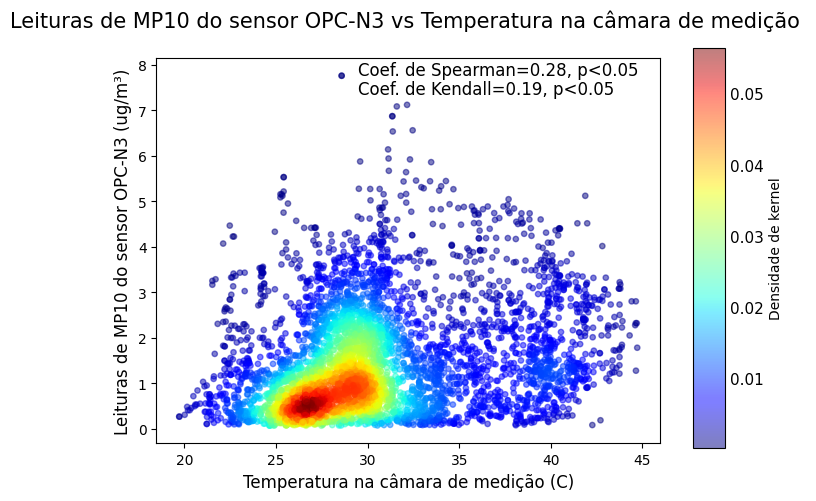
\includegraphics[width=\textwidth]{chapters/3-ANÁLISE DOS DADOS/Figuras/temperature-pm10.png}
        \caption{Relação entre as leituras do sensor OPC-N3 e a temperatura}
        \label{fig:data-temp-pm10-corr}
    \end{subfigure}
    \fonte{Desenvolvido pelo autor (2023)}
\end{figure}

Na Tabela \ref{tab:data-contab-pm10} contabilizam-se os dados para período de 15 minutos e de 1 hora. Observa-se que dos 14541 pontos de dados, que representavam as amostras adquiridas com um período de 15 minutos no intervalo de 21/11/2022 até 21/04/2023, 5668 foram aproveitados como dados válidos, o que representa um 39 \% aproximadamente dos dados originais. Ao re-amostrar esses 5668 pontos em dados horários obtiveram-se 1291 amostras horárias de concentração válidas (aproximadamente 36 \% dos dados) para realizar a calibração. Vale salientar que nos dados de \acrshort{mp10} não foram encontradas alterações na linha base nem dados de estabilização já que esse sensor não precisa desse intervalo prévio as medições.

\begin{table}[h]
    \caption{Contabilização dos dados por etiquetas das leituras do sensor OPC-N3}
    \centering
    \begin{tabularx}{0.95\textwidth}[h]{
         >{\raggedright\hsize=.45\hsize\arraybackslash}X
         >{\raggedright\hsize=.20\hsize\arraybackslash}X 
         >{\raggedright\hsize=.5\hsize\arraybackslash}X
         >{\raggedright\hsize=.50\hsize\arraybackslash}X 
         >{\raggedright\hsize=.20\hsize\arraybackslash}X 
         >{\raggedright\hsize=.5\hsize\arraybackslash}X }
        \multicolumn{3}{c}{Série temporal T = 15 mins} & \multicolumn{3}{c}{Série temporal T = 1 hr} \\
        \hline
        Etiquetas & No. amostras & \% amostras & Etiquetas & No. amostras & \% amostras \\ [0.5ex]
        \hline
        \textit{MISSING} & 6053 & 41.63 \% & \textit{LOWSAMPLES} & 2291 & 63.96 \% \\ [0.5ex]
        
        \textit{LTLL} & 1297 & 8.92 \% & \textit{VALID} & 1291 & 36.04 \% \\ [0.5ex]
        
        \textit{GTUL} & 0 & 0.0 \% & & & \\ [0.5ex]
        
        \textit{STABILIZING} & 0 & 0.0 \% & & & \\ [0.5ex]
        
        \textit{BADSPIKE} & 1332 & 9.16 \% & & & \\ [0.5ex]
        
        \textit{LTQTLE01} & 117 & 0.80 \% & & & \\ [0.5ex]
        
        \textit{GTQTLE99} & 74 & 0.51 \% & & & \\ [0.5ex]
        
        \textit{REBASE} & 0 & 0.0 \% & & & \\ [0.5ex]
        
        \textit{VALID} & 5668 & 38.98 \% & & & \\ [0.5ex]
        \hline
        TOTAL & 14541 & & TOTAL & 3582 & \\
    \end{tabularx}
    \label{tab:data-contab-pm10}
    \fonte{Desenvolvido pelo autor}
\end{table}

\subsubsection{Dependência com a temperatura}

Investigou-se a existência de correlação entre as leituras do sensor de \textit{mp10} e as variações de temperatura medida no interior da câmara de medição. Os resultados dos testes estatísticos de Spearman e Kendall revelaram coeficientes de correlação estatisticamente significativos, conforme se ilustra na Figura \ref{fig:data-temp-pm10-corr}. O coeficiente de Spearman resultou em 0.29 com um valor de p inferior a 0.05, indicando uma correlação estatisticamente significativa entre as leituras dos sensores e a temperatura. De maneira semelhante, o coeficiente de Kendall foi de 0.20, também com p < 0.05, reforçando a presença de uma associação significativa. Ao avaliar a hipótese nula de ausência de correlação, os resultados forneceram evidências para sua rejeição, sugerindo a existência de uma correlação entre as leituras dos sensores de \acrshort{mp10} e as variações de temperatura.